\documentclass[a4paper,11pt]{amsart}

\usepackage[margin=3.5cm]{geometry}
\usepackage{lineno}
\usepackage{amsmath}
\usepackage{amssymb}
\usepackage{graphicx}
\usepackage{caption}
\usepackage{xcolor}
\usepackage{dirtytalk}
\usepackage{colortbl}
\usepackage{booktabs} 

%%%%%%%%%%%%%%%%%%%%%%%%%%%%%%%%%%%%%%%%%%%%%%%%%%%%%%%%%%%%%%%%%%%%%%%%%%%%%%%%
%%% BIBLIOGRAPHY DETAILS
%%%%%%%%%%%%%%%%%%%%%%%%%%%%%%%%%%%%%%%%%%%%%%%%%%%%%%%%%%%%%%%%%%%%%%%%%%%%%%%%

\usepackage[maxcitenames=2,style=authoryear-comp,firstinits=true,citestyle=authoryear,natbib=true,backend=bibtex]{biblatex}
\DeclareNameAlias{sortname}{family-given}
\renewcommand*{\multinamedelim}{\addcomma\space}
\renewcommand*{\finalnamedelim}{~and\space}
\setlength{\bibitemsep}{\baselineskip}
\setlength\parindent{3em}
\setlength\parskip{0.5em}
\renewbibmacro{in:}{}

\AtEveryBibitem{%
  \clearfield{url}
  \clearfield{urlday}
  \clearfield{urlmonth}
  \clearfield{urlyear}
  \clearfield{issn}
  \clearfield{month}
%%%  \clearfield{doi}%
  \clearfield{keywords}
  \clearfield{note}
}

\bibliography{ansorge}



%%%%%%%%%%%%%%%%%%%%%%%%%%%%%%%%%%%%%%%%%%%%%%%%%%%%%%%%%%%%%%%%%%%%%%%%%%%%%%%%
%%% CUSTOM DEFINITIONS
%%%%%%%%%%%%%%%%%%%%%%%%%%%%%%%%%%%%%%%%%%%%%%%%%%%%%%%%%%%%%%%%%%%%%%%%%%%%%%%%

\newcommand{\todo}[1]{\textcolor{red}{$[$#1$]$}}
\newcommand{\quotation}[1]{"#1"}

% TO BE USED IN MATH-ENVIRONMENT 
\newcommand{\SFC}{\mathrm{sfc}}
\newcommand{\p}{\partial}
\newcommand{\gzm}{{\xi}}%{\gamma z_\text{match}}}
\newcommand{\RO}{\mathrm{Ro}}  
\newcommand{\RE}{\mathrm{Re}}
\newcommand{\LR}{\Lambda_\RO} 


\date{\scriptsize Draft - Version \today}
\title{Profiles of Wind Direction and Speed in Turbulent Ekman Flow}
\author{Cedrick Ansorge, Hauke Wurps}

\begin{document} 

\maketitle

\begin{abstract}
  The profiles of wind speed and direction in turbulent Ekman flow
  are formulated based on asymptotic theory and data from direct numerical simulation. 
  %
  The profile of the stream-wise component follows the classical viscous, logarithmic and wake scaling.
  %
  In the outer layer, the velocity component profiles can be described by an Ekman-spiral with adapted
  boundary conditions that result in a reduction of the spiral-like rotation. 
  %
  The span-wise component poses a conceptual challenge to the channel-flow analogy
  in the context of asymptotic matching; it exhibits a mixed scaling in the surface layer, but follows
  outer scaling for most of the outer layer.
  %
\end{abstract}
%
%%%%%%%%%%%%%%%%%%%%%%%%%%%%%%%%%%%%%%%%%%%%%%%%%%%%%%%%%%%%%%%%%%%%%%%%%%%%%%%%
%
\section{Introduction}

Wind veer away from its geostrophic direction is
(i) due to direct frictional effects in the very vicinity of the surface and
(ii) due to turbulence which exerts indirect frictional effects; these effects
cause a slow-down of the mean wind reducing the Coriolis force thus turning the wind
in favor of the pressure gradient force. 
%%
Not only does the veering set the frame of reference for surface layer theory, it also has
effects at small and large scales.
%
From a large-scale perspective, the veering of wind across the planetary boundary layer determines
the amount of cross-isobaric mass-flux, commonly referred to as 'Ekman pumping' \citep{ekman:AMA1905},
and it is thus a key factor in the life-cycle of large-scale synoptic systems.
%
% %% This shear is probably not related to Ekman-turning 
% On the mesoscale, shear in the surface layer a crucial factor for the initiation and sustainment of strong convective events (REFERENCE?).
% 
At the small-scale end, the directional shear of the wind in the upper part of the surface layer
may cause a systmatic yaw for tall wind power generation devices where blades reach into the Ekman layer,
i.e. that part of the boundary layer where the wind starts to turn. 
%
\par
%
Wind veer in the planetary boundary layer is commonly characterized by the surface veering angle $\alpha$
defined as the angle between the negative surface shear stress $\tau_\SFC$ and the geostrophic wind.
%
Surface veering $\alpha$ and geostrophic drag $Z\equiv u_\star/G$, where $u_\star\equiv\sqrt{\nu|\tau_\SFC|}$,
uniquely determine the surface drag $\tau_\SFC$ in a turbulent Ekman flow. 
%
In any quantitative description of the surface layer, the friction velocity $u_\star$ is the dynamic scale
and $\alpha$ defines the alignment of the frame of reference.
%
Knowledge about $u_\star$ and $\alpha$ is thus a pre-requisite for any quantitative theory of the surface layer and a first
attempt in theoretical quantification was undertaken by \citet{rossby:PPO1935} using integral relations in the boundary layer.
%
Asymptotic similarity theory was later used by \citet{tennekes:JAS1973, blackadar:JAS1968},
and--based on his seminal direct numerical simulations (DNS) of Ekman flow--,~\cite{spalart:JFM1989} suggested
a modification to take into account effects of low to intermediate Reynolds numbers.
Later on, constants were re-evaluated with a focus on the atmospheric boundary layer based on
observations \citep{hogstrom:BM1988,hogstrom:BM1996}
and numerical modelling \citep{spalart:PF2008, spalart:PF2009, ansorge:BM2014, ansorge:BM2019}. 
%
\par
%
Attempts were also undertaken to obtain profiles of the wind speed: 
One approach is to match the inner and outer layer at a reference height;
\citet{etling:2002, emeis:2018}  (Sec. 21.10; Eq. 21.48) choose the Prandtl-layer height to match
the wind speed profiles, which, however, requires to externally prescribe the veering $\alpha$ at that height. 
A one-dimensional profile with constant veering is given by \citet[Sec. 3; Eq. 3.1-3.19]{emeis:m2007}. 

\citet{gryning:BM2007} present an extension of the wind-speed profile beyond the surface layer
using a neutral referece profile and a stability correction;
\cite{kelly:BM2010}, based on a probabilistic representation of stratification,
develop a model for the long-term mean windspeed
in the atmospheric boundary layer and compare this with observation at different sites; 
\cite{kelly:WE2016} demonstrate the effect of such improved model for wind-energy applications.
%
In consideration of the large scale separation in geophysical flow, the rotation of the wind in the
surface layer is often assumed negligible, and above investigations merely focus on the wind speed; 
that means, the veering of the wind with height is not described and there is little knowledge on the
profile of the span-wise velocity component and the precise shape of the hodograph in the limit of a
truly neutral Ekman boundary layer.
%
%%% \par  %%%%%%%%%%%%%%%%%%%%%%%%%%%%%%%%%%%%%%%%%%%%%%%%%%%%%%%%%%%%%%%%%%%%%%%%%%%%%%%%
%%% % No discussion of higher-order moments at this stage
%%%
%%% For non-rotating, non-external flows theoretical considerations by Townsend (cite to attached-eddy hypothesis)
%%% have recently been confirmed from both wind-tunnel  experiments and numerical simulation
%%% \cite{ng_comparison_2011,marusic_logarithmic_2013};
%%% this implies that physical models for the second moments (Reynolds stresses) of the flow \ldots.
%
\par %%%%%%%%%%%%%%%%%%%%%%%%%%%%%%%%%%%%%%%%%%%%%%%%%%%%%%%%%%%%%%%%%%%%%%%%%%%%%%%%
%
Ekman-layer models and two-layer models of the ABL take into account rotational effects at higher altitudes,
for instance when the wind speed needs to be evaluated at heights on the order of 100-200\,\mathrm{m},
a particular concern when it comes to wind-power forecasting \citep{optis:BM2014}.
%
Despite rotational effects being considered, the formulation of these models for the outer layer
and analysis of their performance primarily focuses on wind speed.
% 
Still, in \citeyear{jiang:JAS2018}, \citeauthor{jiang:JAS2018}
recognized that the outer part of the Ekman boundary layer receives less attention in comparison
with the surface layer and commence in studying the neutral problem by Large-Eddy simulation (LES).
%
They focus on the wind speed and find an extended logarithmic layer when considering the wind speed instead of
the shear-aligned component, and they eventually demonstrate by means of an analytical model that this vertical
extension of the logarithmic layer may be explained by a transfer of stress to the spanwise velocity component where
it is assumed that the shear vector $\tau(z)$ and stress vectors $(\p_zU,\p_zV)$ are aligned. 
%
\par
%
Turbulent Ekman flow is considered here as a conceptual model of the
homogeneous, stationary atmospheric boundary layer over a flat surface under neutral stratification. 
%
Universal profiles of the wind vector for turbulent Ekman flow not only are a well-described limit
for theoretical exploration or higher-order approaches taking into account possible effects of stratification,
roughness or other physical complications encountered in the realgeophysical system.
%
While, on first sight, the study of such a strongly idealized case appears as an academic problem, it contains the essence
of surface similarity as it is used in most atmospheric models, be it conceptual or numeric ones.
%
For instance, effects of roughness are commonly incorporated by a linear transformation of vertical scale involving the
roughness parameter $z_0$ and for larger roughness also a displacement height~%
\citep{monin:1975,jacobs:AFM1988,hogstrom:BM1988}; 
effects of stability are commonly accounted for by a linearization around the neutrally stratified profile~%
\citep{monin:ARF1970, monin:1975, hogstrom:BM1988, hogstrom:BM1996,sakagami:BM2020}.
%
Furthermure, profiles can serve as better initial condition for numerical simulation of the flow,
to minimize the length of initial transient periods, or as benchmark for turbulence
closures that can be tuned to reproduce the neutral limit case.
%
\par
%
Despite the strong simplifications implied by our choice of set-up, there is no straightforward approach to solving
this conceptually well-defined problem.
%
Large-Eddy simulation not only needs to be tuned for the surface shear stress and veering angle, but it also
relies on sub-grid closures that often assume alignment of the stress with gradients -- a questionable
pre-requisite when the wind rotates with height.
%
\citet{esau:EFM2004} investigated the representation of the Ekman boundary layer by dynamical subgrid closures
and \cite{zikanov:JFM2003} proposed a closure for the wind profile using a linearized representation of the eddy viscosity.
%
Despite advances in analysis of this simplified set-up \citep{jiang:JAS2018}, 
there is yet insufficient understanding for a quantitative generalization of the results to
arbitrary external forcing (manifest in variation of the Reynolds number) -- and indeed the fundamental
questions pertaining to such relatively simple dynamics of turbulence are not reflected in the
research foci of LES for the ABL over the past 50 years \citep{stoll:BM2020}. 
%
\par
% 
At the same time, an increasing amount of high-quality and high-resolution data from turbulence-resolving approaches
is emerging due to recent advances in high-performance computing and its application to geophysical problem sets;
the geophysical range of scale separation, however, is--and it will remain so for the foreseeable future--out of reach
for such simulation \citep{dimotakis:ARF2005}.
%
Here, the routinely employed concept of Reynolds-number similarity can help. It postulates the existence
of \say{\emph{fully developed turbulence}  believed to occur for a sufficiently large but finite Reynolds number}
\citep{barenblatt:PF1995}.
%
(Already in \citeyear{moin:ARF1998}, this in fact lead \citeauthor{moin:ARF1998} to the question \emph{how high a Re is high enough}?) 
%
In fully developed turbulence certain statistics such as dissipation \citep{dimotakis:ARF2005} or profiles of
mean velocity \citep{barenblatt:JFM1993} become independent of the Reynolds number when scaled appropriately while
other statistics, such as the near-wall maximum in velocity fluctuation depend on $\RE$ \citep{baars:JFM2020a} and external
interfaces may exert an impact on near-wall scaling \citep{dasilva:ARF2014}. 
%
It appears that for certain statistics in Ekman flow, fully-developed turbulence is reached with the
Reynolds numbers that became possible with the increasing capabilities of supercomputering over
the past decades.
%
\par
% 
This paper exploits the robust features of mean velocity profiles from direct numerical
simulation across a range of Reynolds numbers to formulate both the stream-wise and span-wise components
of the mean velocity vector as a function of the Reynolds number.
%
%%%%%%%%%%%%%%%%%%%%%%%%%%%%%%%%%%%%%%%%%%%%%%%%%%%%%%%%%%%%%%%%%%%%%%%%%%%%%%%%
\section{Problem Formulation and Numerical Approach}
%%%%%%%%%%%%%%%%%%%%%%%%%%%%%%%%%%%%%%%%%%%%%%%%%%%%%%%%%%%%%%%%%%%%%%%%%%%%%%%%
%
We consider here incompressible, turbulent Ekman flow, that is, the turbulent flow over a flat rotating plate, as
a physical model for the truly neutral atmospheric boundary layer (ABL).
%
The f-plane approximation is applied such that rotation only acts on horizontal velocity components;
we thus neglect rotational effects on the horizontal components of velocity and dynamical effects
due to latitudinal variation of the rate of rotation.
%
%%%%%%%%%%%%%%%%%%%%%%%%%%%%%%%%%%%%%%%%%%%%%%%%%%%%%%%%%%%%%%%%%%%%%%%%%%%%%%%%
\subsection{Notation and Governing Equations}
%%%%%%%%%%%%%%%%%%%%%%%%%%%%%%%%%%%%%%%%%%%%%%%%%%%%%%%%%%%%%%%%%%%%%%%%%%%%%%%%
%
The dimensional velocity vector of the numerical simulations is $\underline{U} = (U_1,U_2,U_3) = (U,V,W)$ over the coordinate system
$Oxyz$, where an approximate alignment (plus/ minus few degrees centigrade) of the direction $Ox$ with the surface shear stress is achieved.
The coordinate $Oy$ points away from the wall,  and $Oz$ points in the span-wise direction normal to $Oxy$.
For analysis of the results, we use two coordinate systems that are
(i)  exactly aligned with the surface shear stress and labelled by an upper index $\alpha$ as in $\underline{U}^\alpha$ for the velocity vector, and
(ii) the coordinate system aligned with the free-atmosphere geostrophic wind labelled by an upper index $G$ as in $\underline{U}^G$.
%
We denote by $u_\star$ the modulus surface friction velocity and let $Z_\star=1/u_\star$ for brevity. 
%
\par
%
We consider the incompressible Navier--Stokes equations for the three velocity components on the f-plane in a framework
that is governed by the physical parameters
(i)   geostrophic wind magnitude $G=\sqrt{G_1^2+G_3^2}$ (where $\mathbf{G}=(G_1,0,G_3)$ is the geostrophic wind vector),
(ii)  Coriolis parameter $f$ (representing the angular rotation), and
(iii) kinematic viscosity $\nu$.
   %
These yield a Reynolds number $\RE$ as non-dimensional parameter governing the system.
%
We use the geostrophic wind as velocity and the Coriolis parameter $f$ as time scale for the non-dimensional framework which implies the Rossby radius $\LR=G/f$ as length scale, such that
\begin{equation}
  \RE=\frac{G \LR }{\nu}. 
\end{equation}
%
\par
%
The non-dimensionalized governing equations read as 
\begin{subequations} 
\begin{eqnarray}
  \frac{\partial u_i}{\partial t} &=& \frac{\p \pi}{\p x_i} - u_j \frac{\p u_i}{\p x_j} + \epsilon_{i2j} (u_j -G_j)   + \frac{1}{\RE} \frac{\p^2 u_i}{\p x_{j}^2} \\ 
  \frac{\partial u_j}{\partial x_j} &=& 0,   
\end{eqnarray} 
\label{eqn:governing} 
\end{subequations}
where $u_i=U_i/G$ are the non-dimensional components velocity, $\pi$ is non-dimensional pressure, and $g_j=G_j/G$ are non-dimensionalized components
geostrophic wind (with $g_{1}^2+g_{3}^2=1$ by construction).
%
These equations are solved inside a bounded cube of size $L_x \times L_y \times L_z$ with periodic boundary conditions in the lateral directions $Oxz$, a no-slip--no-penetration boundary at $y=0$ and
a no-penetration, free-slip boundary at $y=L_y$.
%
%%%%%%%%%%%%%%%%%%%%%%%%%%%%%%%%%%%%%%%%%%%%%%%%%%%%%%%%%%%%%%%%%%%%%%%%%%%%%%%%
\subsection{Numerical Simulations}
%%%%%%%%%%%%%%%%%%%%%%%%%%%%%%%%%%%%%%%%%%%%%%%%%%%%%%%%%%%%%%%%%%%%%%%%%%%%%%%%
The problem is solved numerically by tLab\footnote{https://github.com/turbulencia/tlab},
an open-source tool-suite to simulate and analyze turbulent flows.
% 
We use here a fourth-order--five-step Runge--Kutta integration and sixth-order compact schemes
for spatial derivatives in all directions.
%
The incompressibility constraint is enforced by a fractional step approach where the Poisson equation
for the pressure field is soled to machine accuracy using a combined spectral/compact approach as
described in \citet{mellado:ZaM2012}.
%
\par
%
Simulations used here are shown in Tab.~\ref{tab:sim-setup}.
%
We extend an existing set of simulations for $\RE\in\{125\,000, 281\,250,\ 500\,000\}$ \citep[gray shading; cf.][]{ansorge:BM2014,ansorge:JFM2016} 
by new simulations at higher Reynolds numbers up to $1.28\times10^6$.
%
In total, this yields one order of magnitude variation in terms of the scale separation in the boundary layer.
%
\todo{(new and old) Simulations}
\begin{table}
  \caption{\label{tab:sim-setup} Direct numerical simulation datasets used in this work}
  \begin{tabular}{c r r c c c c c}
    \toprule 
    $\RE_\Lambda$ & $\RE_D$ & $L_{xy}/\Lambda$ & $N_x\times N_y\times N_z$ & $\Delta x^+$ & $\Delta y^+$ & $\left.\Delta z^+\right|_{z=0}$ \\ 
    \midrule
    \rowcolor{gray!30}
       $125\,000$ &    $500$& 1.08 & $2048\times2048\times192$&4.1& 4.1& 1.05\\
    \rowcolor{gray!30}
       $281\,250$ & $   750$& 1.08 & $3072\times3072\times384$&5.6&11.2& 1.60\\
    \rowcolor{gray!30}
       $500\,000$ & $1\,000$& 1.08 & $3072\times6144\times512$&9.3& 4.7& 1.14\\
    \midrule
       $845\,000$ & $1\,300$& 0.54 & $2560\times5120\times640$&8.9& 4.5& 0.99\\

    $1\,280\,000$ & $1\,600$& 0.54 & $3860\times7680\times960$&8.6& 4.3& 1.00\\ 
    \bottomrule 
  \end{tabular} 
\end{table}
%
%%%%%%%%%%%%%%%%%%%%%%%%%%%%%%%%%%%%%%%%%%%%%%%%%%%%%%%%%%%%%%%%%%%%%%%%%%%%%%%%
\section{Overview of the new simulations at $\RE_\tau$ up to 3000}
%%%%%%%%%%%%%%%%%%%%%%%%%%%%%%%%%%%%%%%%%%%%%%%%%%%%%%%%%%%%%%%%%%%%%%%%%%%%%%%%
%
Uniqueness and necessity of new simulations
%
\par
%
PARAGRAPH ON BULK PARAMETERS AND SCALING (cf. \ref{tab:bulk_results})
\begin{table}
  \caption{Bulk characterization of the simulations \label{tab:bulk_results}}
  \begin{tabular}{r r r r r r r }
    \toprule
    Re & $\delta^+=\RE_\tau$& $u_\star$ & $\alpha$ & $\delta_{95}/\delta$ & $f u_\star^{-3}\int_{0}^{\delta} e \mathrm{d} z $ & $ G^{-3}\int_{0}^{\delta} \epsilon \mathrm{d}z$\\
      \midrule 
      \rowcolor{gray!30} 
      500 & 479 & 0.0619& 25.5 & 0.66& 0.88& 1.31 \\
      \rowcolor{gray!30} 
      750 & 886 & 0.0561& 21.0 & 0.65& 0.90& 1.34 \\
      \rowcolor{gray!30}
      1000& 1403& 0.0530& 18.8 & 0.62& 0.92& 1.30 \\
      \midrule
      1300& 2122& 0.0501& 17.9 & 0.59& 0.85& 1.24 \\
      1600& 2978& 0.0482& 17.2 & 0.61& 0.91& 1.21 \\ 
      \bottomrule
    \end{tabular}
\end{table} 
%
\par
%
PARAGRAPH ON VELOCITY AND STRESS PROFILES cf. \ref{fig:stresses}
\begin{figure}
  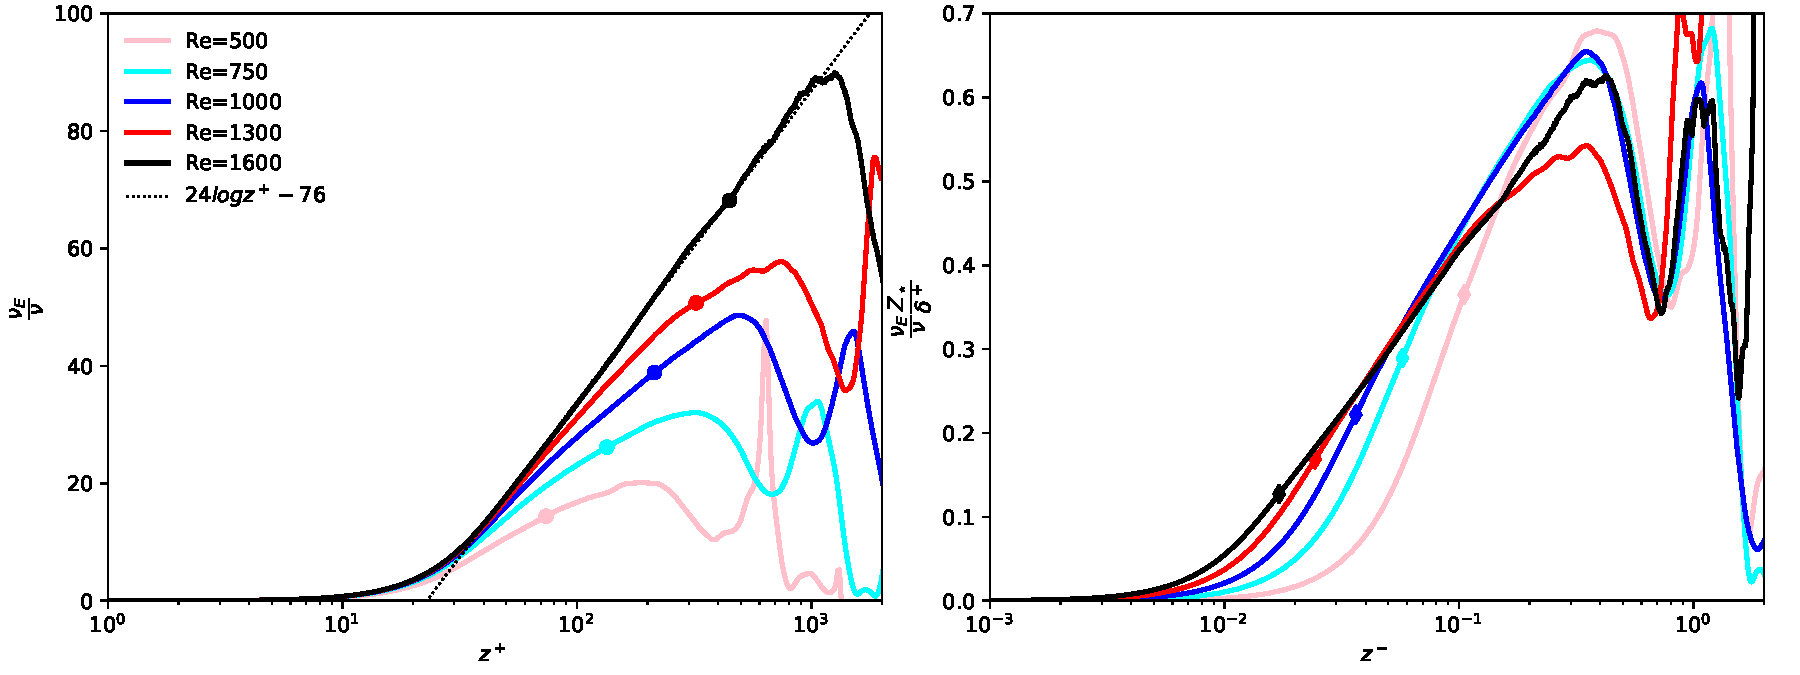
\includegraphics[width=0.66\textwidth]{../plot/eddy_viscosity.pdf}
  \caption{Reynolds stresses and eddy viscosity across the Ekman layer plotted in ineer scaling for
    various Reynolds number
    \label{fig:stresses}} 
\end{figure} 
%
\par
%
PARAGRAPH ON TURBULENCE STRUCTURE (2D SLICES, SPECTRA?) cf. Fig.~\ref{fig:slices}  

\begin{figure}
  \centerline{\includegraphics[width=0.33\textwidth]{../plot/PLANES/tke_xz_10.pdf}
  \includegraphics[width=0.33\textwidth]{../plot/PLANES/tke_xz_50.pdf}
  \includegraphics[width=0.33\textwidth]{../plot/PLANES/tke_xz_400.pdf}}
  \centerline{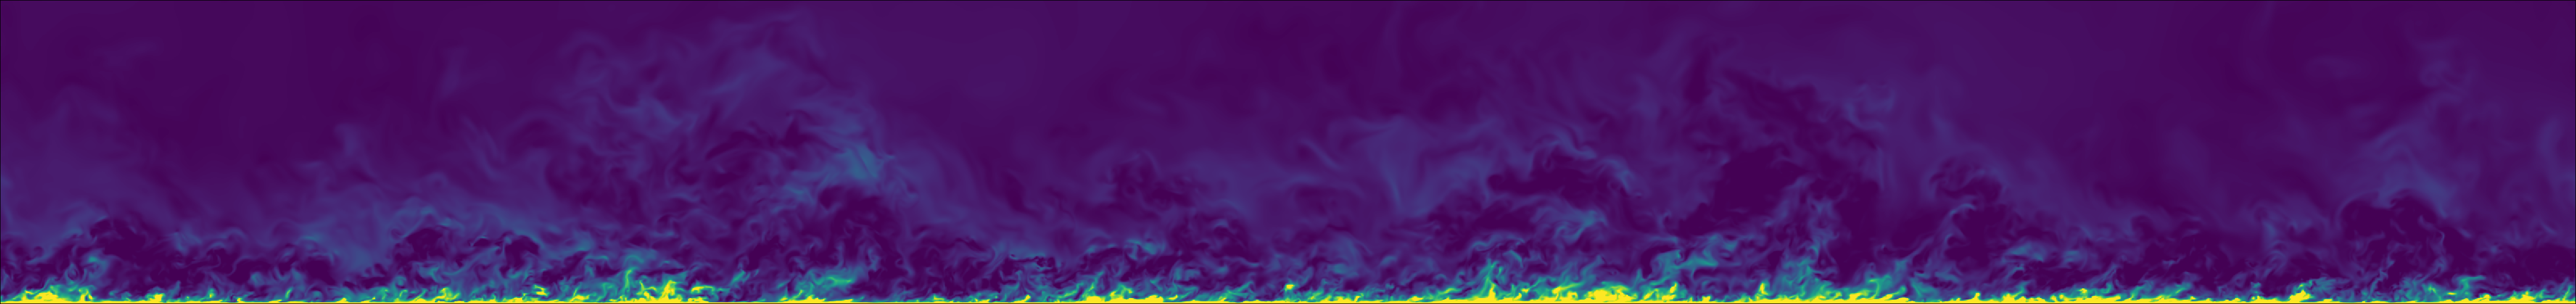
\includegraphics[width=\textwidth]{../plot/PLANES/tke_xy_1.pdf}}
  \caption{horizontal slices of turbulence kinetic energy in the Buffer layer (i=10), Logarithmich Layer (i=100) and outer lzayer (i=400); coloring between percentiles 4 and 96 of the respective image. Lower panel:streamwise--vertical intersect through the domain} 
  \label{fig:slices} }
  
\end{figure} 

%%%%%%%%%%%%%%%%%%%%%%%%%%%%%%%%%%%%%%%%%%%%%%%%%%%%%%%%%%%%%%%%%%%%%%%%%%%%%%%%
\section{Towards a Universal Velocity Profile for the Turbulent Ekman Layer}
%%%%%%%%%%%%%%%%%%%%%%%%%%%%%%%%%%%%%%%%%%%%%%%%%%%%%%%%%%%%%%%%%%%%%%%%%%%%%%%%
%
Formulations for the outer layer that take into account the rotation, and thus deviation from the channel-flow analogy
need to be matched to the framework of surface similarity, and it
occurs that a smooth transition from the inner to the outer layer is not easily achieved.
%
\cite{optis:BM2014}, for instance, define an ``effective geostrophic wind vector that has the same magnitude of the
observed surface geostrophic wind and is rotated by the angle $\alpha$ [their nomenclature]'' to overcome the
unsteady transition when coming approaching the Ekman layer from below.
%
While such rotation of the wind vector is \emph{a posteriori} justified by the observational data that the model outcomes are compared to,
we believe that it is the manifestation of a mismatch between the theoretical treatment of the inner and outer layer of
turbulent Ekman flow.


\end{itemize}
\begin{figure}
  \centerline{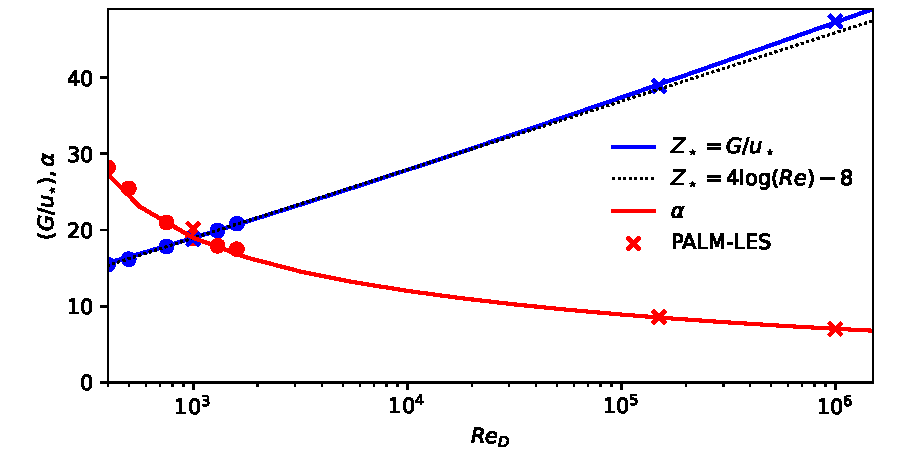
\includegraphics[width=0.7\textwidth]{../plot/ustar_alpha.pdf}}
  \caption{Variation of geostrophic drag, $Z_\star$, and surface veering, $\alpha$, with Reynolds number according to
    the theory by Spalart et al. (1989) and as estimated from DNS data}
  \label{fig:drag_law}
\end{figure}
% 
\subsection{Drag-Law}
A drag-law for Ekman flow determines two key parameters of the flow as a function of Reynolds number alone.
%
These are, first, the modulus of the surface friction normalized by the geostrophic wind forcing, $u_\star$ and,
second, the direction of surface shear stress, $\alpha$, also termed wind veering. 
%
A non-zero veering of the wind is a rather special case in comparison with most turbulent flows conisdered in an
engineering context, and it confronts us with a situation where the most appropriate coordinate system for analysis
(namely that aligned with the surface shear stress) is a priori unknown. 
%
We compare our DNS data against a semi-empirical drag-law based on integral consideration \cite{spalart:JFM1989}
and find, as demonstrated in previous work \cite{ansorge:BM2014}, excellent agreement in the range
 $400<\mathbf{Re}<1600$, representing a factor of 16 in variation of viscosity. 
%
\par
%
We also find that the solution of the transient equation involved in estimation of $u_\star$ for a given Reynolds number
$Re_D$ is approximated reasonably by the formulation
\begin{equation}
  u_\star= 4\log(\mathbf{Re}_D))-8
\end{equation}
which quantifies the 'weak' dependence of $u_\star$ on the Reynolds number as an approximately logarithmic one, at least
for problems with a scale separation on the order that is relevant to geophysical problems ($Re_D<10^{8}$).  
%
%%%%%%%%%%%%%%%%%%%%%%%%%%%%%%%%%%%%%%%%%%%%%%%%%%%%%%%%%%%%%%%%%%%%%%%%%%%%%%%%
%
\subsection{Profile in the outer layer}
%
The outer layer of Ekman flow is characterized by a turning of the wind velocity and the super-geostrophic maximum
that is sustained by momentum convergence at the inflection point of the velocity profile. 
The super-geostrophic maximum of streamwise velocity and a secondary minimum aloft the bulk-turbulent part of
the boundary layer are well-described by a classic Ekman spiral with adapted boundary conditions and a shift
in reference height.
%
\begin{figure}
  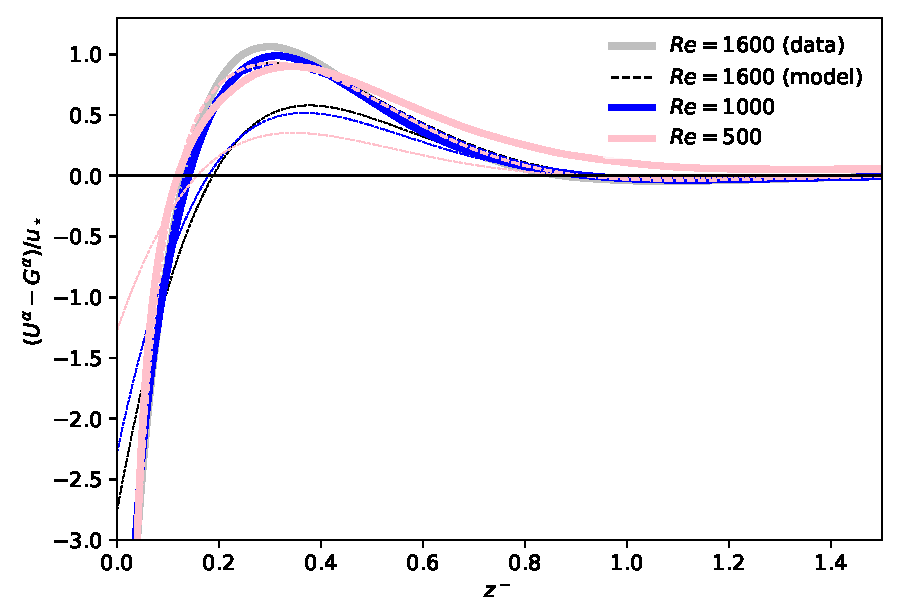
\includegraphics[width=0.5\textwidth]{../plot/outer_layer_u.pdf}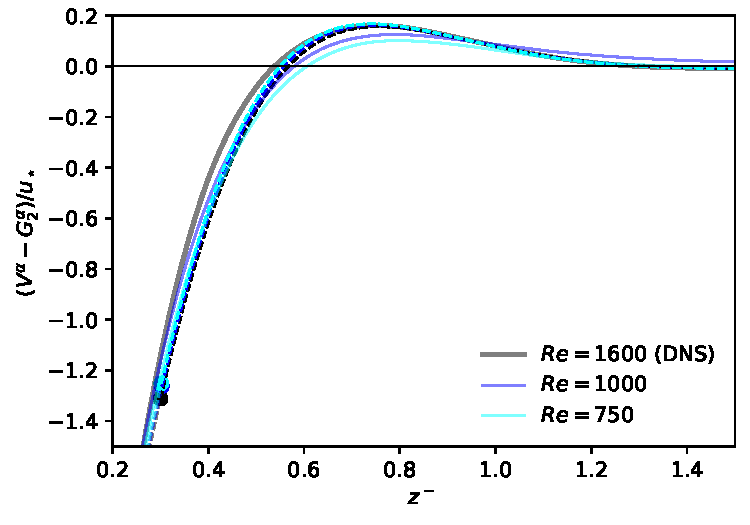
\includegraphics[width=0.5\textwidth]{../plot/outer_layer_w.pdf}
  \caption{} 
\end{figure}

\subsection{Stream-wise Velocity Component} 
For the stream-wise velocity profile (that in non-rotating flows due to the geometry is always aligned with the surface shear stress),
well-established theories exist for various regimes according to their distance from the wall and the relative role of
viscosity, turbulence and interaction with the outer region of the flow with the logarithmic law for the mean velocity as a central anchor point.
%
\par
%
\begin{subequations}

In immediate vicinity to the surface, local turbulent mixing cannot occur for the no-slip/no-penetration boundary condition,
and the mean velocity is described by a viscous profile of the form
\begin{equation}
  (U,W)^{\alpha+}  = (z^+,0)  
\end{equation}
where the direction of the velocity points into the exact opposite direction of the wall shear stress $\tau$. 
In absence of roughness elements and for small roughness ($z_0^+<5$), this linear regime is known as
viscous sub-layer \cite{foken:m2002,foken:BM1978}.
In fact, this law of the wall has no degree of freedom given the drag, i.e. once $u_\star$ and $\alpha$ are defined. 
%
However, theoretical foundation is lacking for the exact shape of the velocity profile in the buffer layer; though crucial for turbulence
production, it is commonly understood as a transition region between the linear profile at the surface and the logarithmic profile
aloft.
A pure blending from the linear velocity profile into the logarithmic one is, however, not reasonable as both the linear and logarithmic
profile overestimate the velocity in the buffer layer. We therefore introduce a higher-order compensating term into
the linear profile before blending it into the logarithmic law:
\begin{equation}
  U_\text{inner}^{\alpha}^+ = \frac{ y^+ + \gamma_4 (y^+)^{4} + \gamma_6 (y^+)^{6} } { 1 + \gamma_6 /u_{ref} (y^+ )^6}, 
\end{equation} 
where the fourth- and sixth-order terms in the nominator are designed to fit the profile below $y^+\approx 10$ and
the sixth-order correction in the denominator limits the growth of $u_\text{inner}$ for large $y^+$.
%
\par
%
In the logarithmic region, we use the profile
\begin{equation}
  U_\text{log}^{\alpha}^+ = \frac{1}{\kappa} \log y^+ + C 
\end{equation}
with the von-K\'arm\'an constant $\kappa=0.416$ and the boundary condition $C=5.4605$. %  log-layer (K\'arm\'an, Prandtl, Jimenez, Marusic)
%
\par %%%%%%%%%%%%%%%%%%%%%%%%%%%%%%%%%%%%%%%%%%%%%%%%%%%%%%%%%%%%%%%%%%%%%%%%%%%%%%%%
%
\end{subequations} 
%
\begin{figure}
  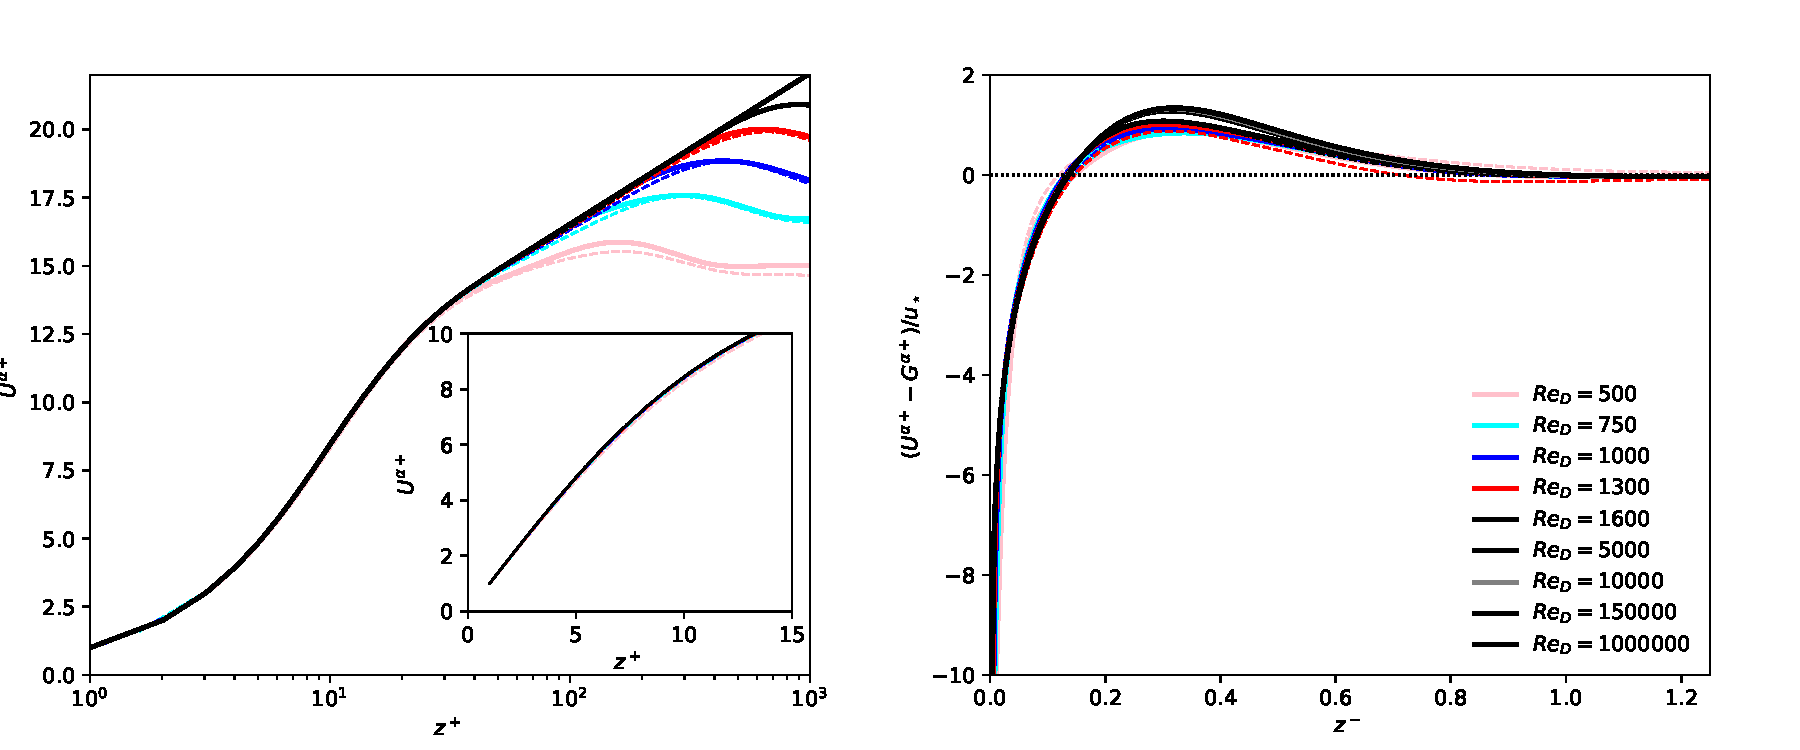
\includegraphics[width=\textwidth]{../plot/u_profile.pdf}
  \caption{Shear-aligned profiles of velocity components $U^{\alpha+}$ in inner (left) and outer (right) units.} 
\end{figure} 
%
%%%%%%%%%%%%%%%%%%%%%%%%%%%%%%%%%%%%%%%%%%%%%%%%%%%%%%%%%%%%%%%%%%%%%%%%%%%%%%%%%%%
%
\subsection{Span-wise velocity}
%
%%%%%%%%%%%%%%%%%%%%%%%%%%%%%%%%%%%%%%%%%%%%%%%%%%%%%%%%%%%%%%%%%%%%%%%%%%%%%%%%%%%
%
The background rotation and associated veering of the surface wind implies a non-zero profile for the span-wise
velocity which challenges the conventional assumptions related to the so-called channel-flow analogy:
%
While the universal profiles in vicinity of the wall implies that the profile be zero or at least small with respect to the stream-wise
component, the veering requires a value of $V_{top}=U_G\sin\alpha$ in the free stream (and thus also at the top of the boundary layer if we assume
that substantial velocity gradients are confined to the turbulent part of the flow). 
%
This is commonly shown in terms of velocity hodographs aligned with the outer, geostrophic flow (cf. Fig.~\ref{fig:hodograph}) and normalized by
the geostrophic wind. 
%
Thus, the drag-law already implies three important properties of these hodographs,
(i) the boundary conditions at the surface,
(ii) the boundary condition at the top, and
(iii) the inclination of the hodograph at the origin by the surface veering:
\begin{subequations} 
\begin{eqnarray} 
 \underline{U}^{G}(z=0) &=& 0,\\ 
 \underline{U}^{G}(z\mapsto\infty) &=& \underline{G}^G = \left(\begin{array}{c}1\\0\end{array}\right) \\
   \left.\frac{\partial V^G}{\partial U^G}\right|_{z=0} &=& \sin\alpha
\end{eqnarray} 
\end{subequations} 
%
Outer scaling of the velocity profile further implies that the velocity deficity of the spanwise component $V^\alpha-G^\alpha$
be a universal function of the outer height $z^-$, i.e.  
\begin{eqnarray}
  V^\alpha-G^\alpha = f^\alpha_V(z^-).  
\end{eqnarray}
%
Interpreting the shear-aligned spanwise velocity deficit $f_{V}^{\alpha}(z^-)$ as 
a signature of outer rotation may lead one to conclude that this universal function
is appropriate down to the surface--irrespective of the Reynolds number.
%
This cannot be the case for the variation of $f_{V}^{\alpha}(z^-)$ across the boundary layer (i.e. between $0<z^-<1$)
must fulfill the drag law and boundary conditions;
at the same time, the weak dependence of $\alpha$ and $u_\star$ on $Re$ implies this range depends on $Re$.
%
%%%PAR
%
\paragraph{Outer Layer.} In the outer region of the flow (for $z^-\mapsto 1$), $f_V(z^-)$, should govern the
spanwise velocity profile which indeed is supported by our DNS data (Fig.\ref{fig:outer_w}):
%
The deficit is close to zero for $z^-\gtrsim 1$, and can be approximated by a logarithmic profile in the
range $0.15\lesssim z^- \lesssim 0.4$.
%
The slope of this profile is best fit by $\kappa_V=0.836 (1 + 150 / Re_D) \kappa$, where the correction term for low Reynolds number
may be omitted for $Re_D \gg 1000$.
%
Based on Fig.~\ref{fig:outer_w}, we pick the offset as
a constant fraction (0.906) of $V^\alpha_G=Z_\star \sin\alpha$, i.e
\begin{subequations} 
\begin{align}
  V_\text{log}(z^-)  = \frac{1}{\kappa_V} \log\left(\frac{z^-}{0.4}\right) + 0.906V_G^{\alpha}. 
\end{align} 
%
%%%PAR
% 
The eventually converged simulations at intermediate $Re_D$ (where the DNS could be run over several inertial periods)
exhibit a super-geostrophic maximum (positiv velocity deficit) in the span-wise component.
%
This maximum is not present or less pronounced for the simulations at higher $Re$ where closer analysis reveals that the
velocity profiles in the outer layer are still subject to a small though finite adaptation process on the inertial time
scales $2\pi/f$ due to the relatively short time span for which these cases could be simulated.
%
While there is no physical model for this wake region that leads to an analytical velocity profile formulation in the span-wise direction,
an error-function transition from the outer logarithmic law to the boundary condition provides a reasonable fit:
%
\begin{align}
  V_\text{outer}(z^-) = (1-w_V)V_\text{log}(z^-) + w_V V_G^\alpha
\end{align} 
with
\begin{align} 
w_V = \frac{\mathrm{erf}\left[\xi_\text{outer} \log(z/z_\text{ref})\right]  + 1}{2}
\end{align}
where $\xi_\text{outer}$ is a transition scale that defines the width of the wake region and $z_\text{ref}$ defines the height.
Based on the DNS data, we choose $\xi_\text{outer}=2$ and let $z_\text{ref}$ such that $V_\text{log}(z_\text{ref}) = 0.98V_G^\alpha$.
There is, however, a degree of ambiguity in the exact choice of these parameters due to the imperfect convergence of the
DNS data to the statistical equilibrium.
%
\end{subequations} 
%
%%% PAR
%
\subsub{Inner Layer.} It is important to note that the logarithmic layer observed here for the spanwise velocity does not
conincide with the log-region of the streamwise velocity but is rather a 'continuation' through the outer layer.
%
This is consistent with the recent finding of a second log-region in the outer region of Ekman flow
(... et al. (incl. Sullivan), JAS 2019).
%
Below this region, the gradients in span-wise velocity are rather small and the span-wise velocity
monotonically approaches its surface boundary condition $V(z=0)=0$.
%
While the stream-wise velocity follows a universal inner scaling that has acquired its universal, $Re$-independent shape for $Re_D> \mathcal{O}\left(10^3\right)$, the span-wise component that defines how the velocity vector veers when the surface is approached,
does not collapse in inner units, and there is, most importantly no sign of convergence even at the highest Reynolds numbers for
which simulations where carried out.
%
Even though the simplest assumption $V=0$ is reasonable for the lower part of the surface surface layer ($z^-<10^{-3}$), it does
not appropriately capture the profile in the rest of the surface layer:

First, $V=0$  implies a discontinuity in the velocity profile at $z^-=0.1$, where the outer scaling found above 
yields a finite value at geophysical $Re$, i.e. there is non-zero veering in the upper part of the
surface layer--as is well-known also from field observation. 
%
Second, the layer around $z^-=0.1$ is crucial to obtain the characteristic and well-established shape of the hodographs as the layer
where $V$ sets in marks the 'maximum' of $V^-$ vs. $U^-$.
%
This illustrates that the higher-order (in terms of the channel-flow analogy where $V=0$) correction follows a mixed scaling when the surface is
approached which has been demonstrated for higher-order terms in other types of flow \citep{mellado:BM2016}. 
%
\par
%
The scale for the magnitude of the span-wise velocity component is $u_\star\sin\alpha$. 
%
Based on our DNS data, we suggest that the Reynolds number scaling of this velocity-magnitude scale is captured
by $Re_\tau^{-1/2}$ which is indeed known from the generalization of higher-order statistics, such as turbulent fluxes
in the inner layer \citep{marusic:JFM2013} that also follow a mixed scaling in the inner layer.
%
We then parameterize the spanwise velocity at 10 wall units as anchor point in the inner layer:
\begin{subequations}
\begin{align}
  V_{10}\equiv V(z^+=10)=750 \frac{u_\star\sin\alpha}{\sqrt{Re_\tau}}.
\end{align} 
%
This leaves us with three fixed points of the velocity profile in the inner layer, namely
(i) the boundary condition $V_0=0$,
(ii) $V_{10}$ at $z^+=10$, and 
(iii) the lower end of the logarithmic profile at $z^-=0.1$ where the latter two are semi-empirically estimated
from DNS data. 
%
In absence of well-established scaling considerations for the span-wise velocity, the choice of profile fits joining
these three points is indeed arbitrary, but we can resort to the DNS data for an empirical approach and find
that a square-root profile fits $V(z^+)$ in the surface layer.
%
A linear profile for $V$ is employed in the viscous sub-layer.
%
Based on the physical extent of the viscous sub-layer in Ekman flow around five wall units \citep{foken:m2002, ansorge:BM2019},
we choose $z^+=5$ to transition from one to the other and note that $V$ is already very small at this height.
%
The span-wise velocity profile in the surface layer is then estimated as 
\begin{align}
  \left.V(z^+)\right|_{\text{inner}} = \left\{\begin{array}{c c l}
  a_1 z^+&;& z^+ \le 5\\ 
  b_1+b_2 \sqrt{z^+}&;& 5<z^+<Re_\tau/10 
  \label{eqn:w_profile_inner}
  \end{array} \right, 
\end{align}
with $b_1$ and $b_2$ estimated such that
\begin{eqnarray}
  \begin{array}{r c l} 
    \left.V(z^+=10)\right|_\text{inner}&=&V_{10}\\
    \left.V(z^+=Re_\tau/10)\right|_\text{inner}&=&V_{\text{outer}}(0.1)\\
  \end{array}
  \Rightarrow \left\{ \begin{array}{l}
    b_2=\dfrac{V_\text{outer}(0.1) - V_{10}}{\sqrt{Re_\tau/10}-\sqrt{10}}  \\[1.5em]
    b_1= V_{10} - \sqrt{10}b_2
  \end{array}\right. 
\end{eqnarray}
We then estimate $\alpha$ from the matching condition at $z^+=5$, i.e.
\begin{align}
  5a = b_1+\sqrt{5}b_2 \Rightarrow a = \frac15 \left[V_{10} + (\sqrt{5}- \sqrt{10})\left(\frac{V_\text{outer}-V_{10}}{\sqrt{Re_\tau/10}-\sqrt{10}}\right) \right].
  \label{eqn:alpha_coefficient} 
\end{align}
%
%%%PAR
%
\paragraph{Matching region.} While the profile composed of $V_\text{inner}(z^+\le 0.1 Re_\tau)$, $V_\text{outer}(z^->0.1)$ is continuous,
it is not smooth at $z^-=0.1$, i.e. at the transition from power-law ($V\propto \sqrt{z^+}$) to logarithmic scaling.
%
To alleviate this issue, we use a second-order polynomial for transition from the inner to the outer layer in the range
$z_\text{low}<z<z_\text{up}$ such that
\begin{align} 
  V_\text{trans}(z^-) &=& V_\text{inner}(z^+_\text{low}) + \Delta V \left(a z_{arg} + b (z_{arg})^2\right)
\end{align}
with $\Delta V &=& V_\text{outer}(z^-_\text{up})-V_\text{inner}(z^+_\text{low})$
and  $z_{arg} = (z - z_\text{low})/(z_\text{up}-z_\text{low})$.
It is  $a+b=1$ for $V_\text{trans}(z^-_\text{up}) = V_\text{outer}(z^-_\text{up})$, and we constrain $a$ by
\begin{align}
  \left.\frac{\partial V_\text{trans}}{\partial z^-}\right|_{z=z_\text{low}} = \left.\frac{\partial V_\text{inner}}{\partial z^-}\right|_{z=z_\text{low}},
\end{align}
where we find that $z^-_\text{low}=0.06$ and $z^-_\text{up}=0.13$ yield satisfactory agreement with DNS data. 
 
%
\begin{figure}
  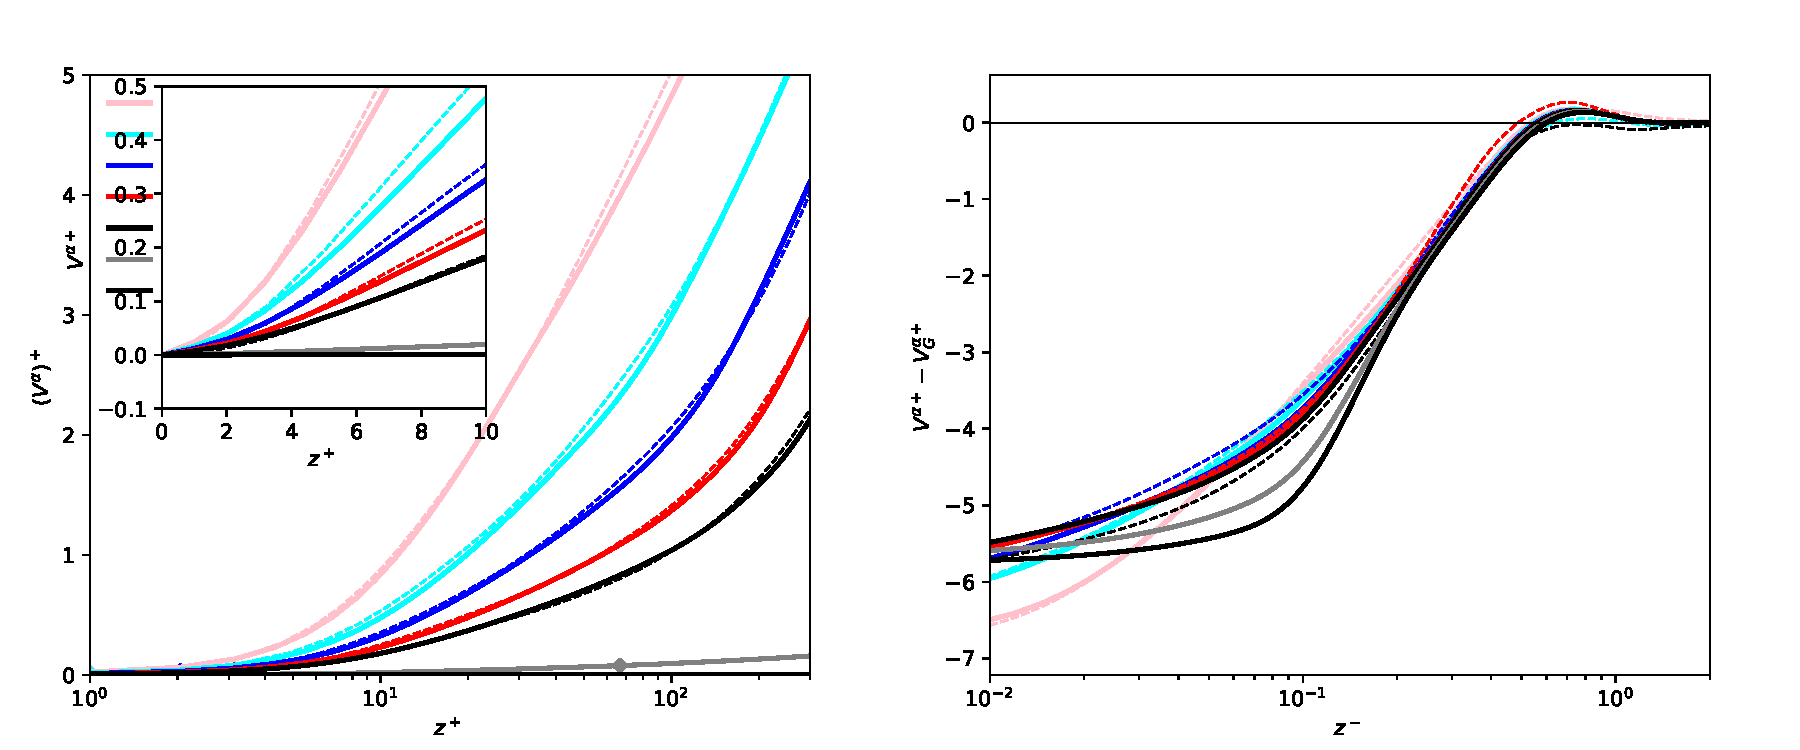
\includegraphics[width=1.0\textwidth]{../plot/w_profile.pdf}
  \caption{Profiles of shear-aligned span-wise velocity $(W^\alpha)^+$ versus inner and outer height.
  Dashed lines show DNS data, thick, opaque lines are from the semi-emprical theory developed above. }
  \label{fig:outer_w} 
\end{figure}
\end{subequations}



\begin{figure}
  \phantom{AAA}\textbf{(a)\hspace{0.3\textwidth}(b)\hspace{0.3\textwidth}(c)}\\
  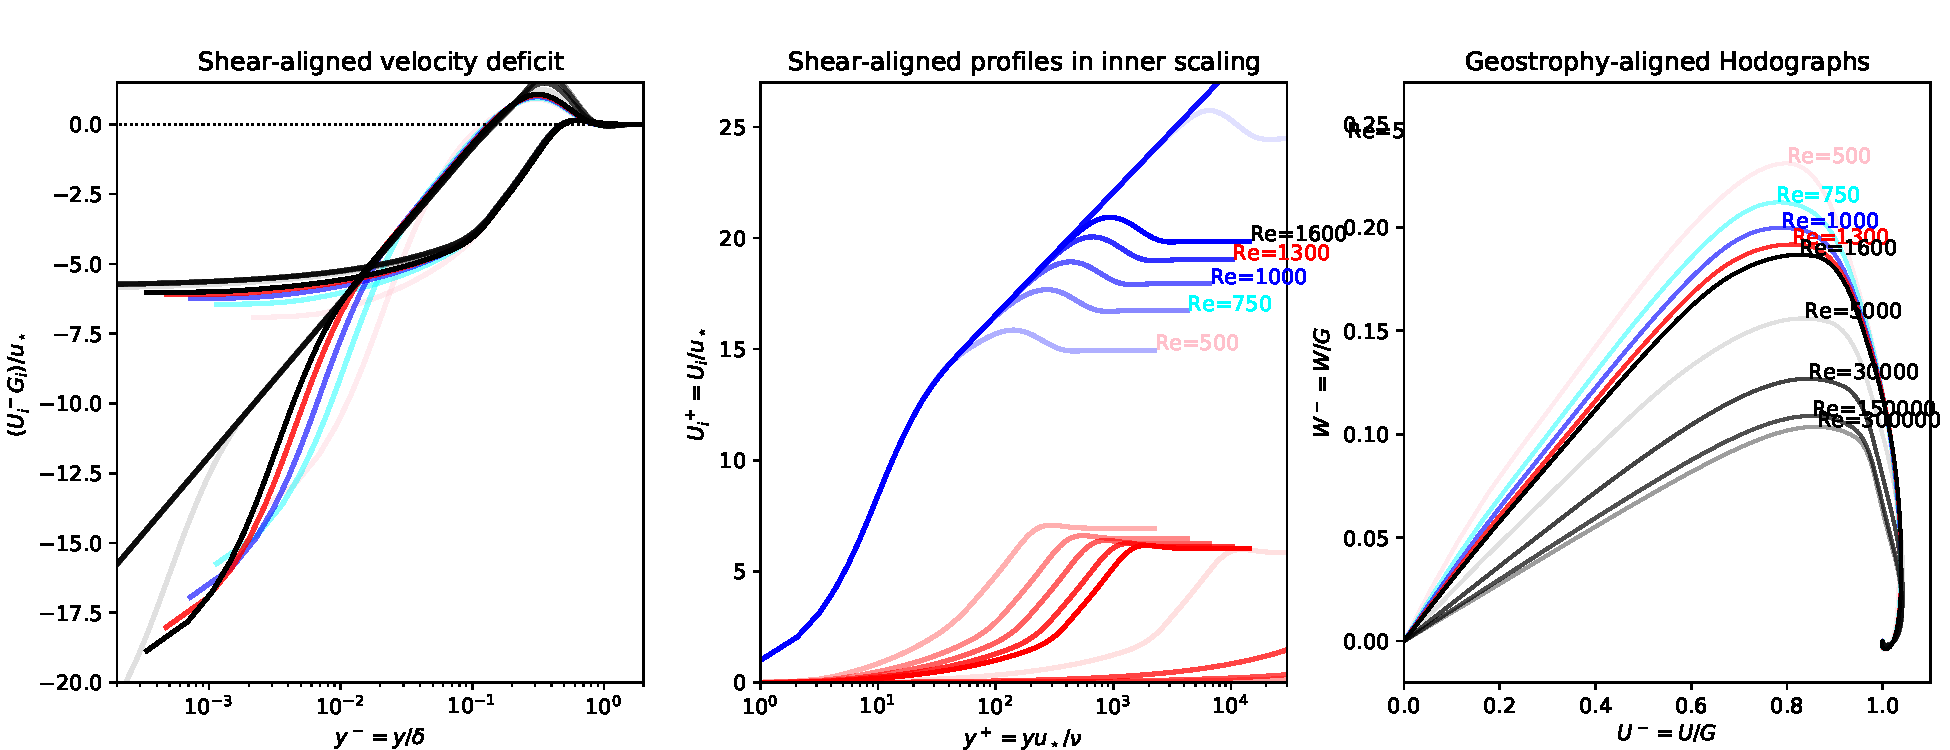
\includegraphics[width=\textwidth]{../plot/ekman_profiles.pdf}
  \caption{ \textbf{(a)} Velocity deficity, \textbf{(b)} velocity profile in shear-aligned hodographs and \textbf{(c)} hodograph in geostrophy-aligned coordinates.
    Thick, solid lines show theory, dashed lines data from DNS. }
  \label{fig:hodograph} 
\end{figure} 

\section{Comparison with other theories}

\textbf{Compare} to Emeis (2002) and Gryning (2007); highlight explicit knowledge on veering-profile $\rightarrow$ directional sheer;
%
\par%%%%%%%%%%%%%%%%%%%%%%%%%%%%%%%%%%%%%%%%%%%%%%%%%%%%%%%%%%%%%%%%%%%%%%%%%%%%%%%%
%
Implications for \textbf{K-theory} (we now can consider that shear and stress are not necessarily perfectly aligned).
$\rightarrow$ can we do something to infer a K-profile from these theoretical considerations? 
%
\begin{figure}
  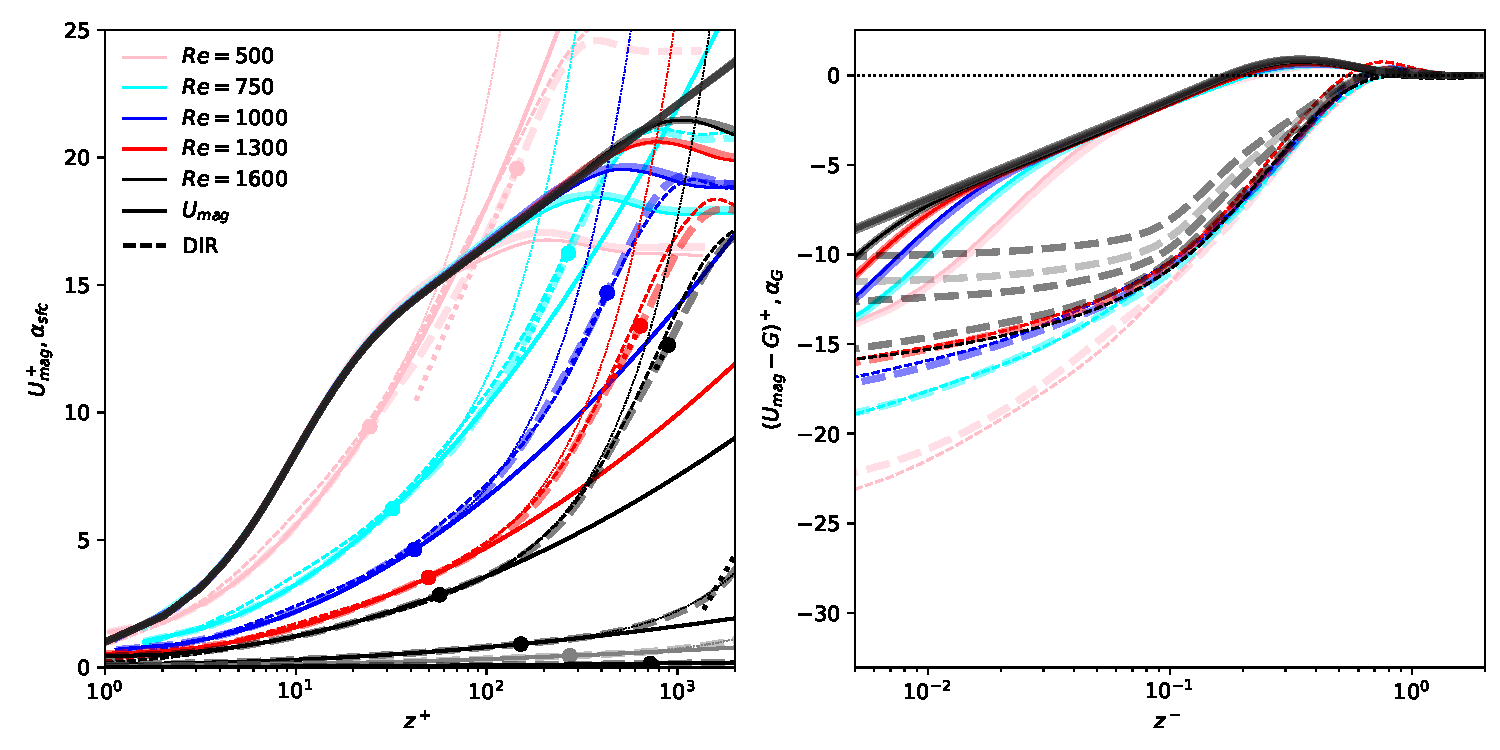
\includegraphics[width=\textwidth]{../plot/mag_dir.pdf} 
  \caption{Total velocity and veering (in degrees) vs inner and outer height.
    Dashed lines show DNS data, thick lines are from semi-empirical theory.} 
\end{figure} 
%
\section{Conclusions}
%
Applications:
\begin{itemize}
\item reference-shear for neutral profile approaches(systematic!) $\rightarrow$ wind engineering! 
\item initial condition for LES/DNS to eliminate/minimize inertial oscillation in Benchmark simulations
\item
\end{itemize} 

\appendix

\section{Laminar Ekman solution with consideration of inner layer}

\begin{subequations}
\begin{eqnarray}
  \left(\begin{matrix}
    \p_t U\\
    \p_t W  
  \end{matrix}\right)&=&\left(\begin{matrix}
     fW &+& \nu \p_z^2 U\\ 
    -f(U-G) &+& \nu \p_z^2 W
  \end{matrix}\right)\\ 
  \Rightarrow \partial_t (U+iW) &=& f(W-i(U-G))) + \nu \p_z^2(U+iW)
\end{eqnarray}
In stationary conditions, this system is solved by
\begin{eqnarray}
  \hat{u}(z) &=& U_{\infty} + e^{-\gamma z} \left[A \cos\gamma z + B \sin\gamma z\right]   \\
  \hat{w}(z) &=& W_{\infty} + e^{-\gamma z} \left[-A \sin\gamma z + B \cos\gamma z\right]
\end{eqnarray} 
\end{subequations}
where the constants $U_\infty$, $W_\infty$ set the top boundary condition and $A$ and $B$ set the bottom boundary condition. 
%
The most common boundary condition for a surface Ekman layer is $A=U_{\infty}=G$, $B=0$, and $W_{\infty}=0$.
%
The lower boundary condition, however, neglects the existence of the surface layer, and it appears reasonable to define
$A=c G$ where $c<1$ is a constant that icorporates the increased shear in the surface layer.
%
Given a 'matching height' $z_{match}$ and normalized matching height $\xi=\gamma z_\text{match}$ in the upper part of the inner layer, we can match the Ekman profile
to the inner layer by letting
%
\begin{eqnarray}
  \begin{matrix} 
    u(z_\text{match}) \equiv u_\text{match} &=& U_{\infty} + e^{-\gzm}} \left [ A \cos\gzm + B\sin\gzm \right] \\
    w(z_\text{match}) \equiv w_\text{match} &=& W_{\infty} + e^{-\gzm}} \left [-A \sin\gzm + B\cos\gzm \right]
  \end{matrix} 
\end{eqnarray}
\begin{eqnarray}
  \Rightarrow \left(\begin{matrix}
    u_\text{match}-U_{\infty} \\ 
    w_\text{match}-W_{\infty}
  \end{matrix}\right) = e^{-\gzm}\left(\begin{matrix}A \\ B \end{matrix}\right)\left(\begin{matrix}
    \cos\gzm &+ \sin\gzm \\ -\sin\gzm &+ \cos\gzm
  \end{matrix} \right) \\
\end{eqnarray}
Matching the profile at $\xi=0$, one obtains
$A = \Delta u_\text{match} $ and $B=-\Delta w_\text{match} $; and when the direction $Ox$ is aligned
with the geostrophic wind, we obtain the textbook-case $A=|\mathbf{G}|$ and $B=0$. 

Otherwise, choosing $B \ne 0$ allows to introduce a phase shift of the Ekman rotation with respect to
the decay of the wind spiral.
%
As, however, in our context, the thickness and position of the spiral can already be controlled by
the eddy viscosity and an offset in $\zeta$, here we let $B=0$.
%%%%%%%%%%%%%%%%%%%%%%%%%%%%%%%%%%%%%%%%%%%%%%%%%%%%%%%%%%%%%%%%%%%%%%%%%%%%%%%%
%% Determining parameters A and B from profile values at a given height
%%%%%%%%%%%%%%%%%%%%%%%%%%%%%%%%%%%%%%%%%%%%%%%%%%%%%%%%%%%%%%%%%%%%%%%%%%%%%%%%
%% 
%% \begin{subequations} 
%% \begin{eqnarray}
%%   e^\gzm \Delta u_\text{match} = A \cos\gzm + B\sin\gzm \\
%%   e^\gzm (\cos\gzm \Delta u_\text{match} - \sin\gzm \Delta w_\text{match}) = A (\cos^2\gzm + \sin^2\gzm)
%% \end{eqnarray}
%% \begin{eqnarray}
%%   \Rightarrow A &=&e^\gzm (\cos\gzm\Delta u_\text{match} + \sin\gzm \Delta w_\text{match})\\
%%   B&=&  \frac{e^\gzm \Delta u_\text{match} - A \cos \gzm}{\sin\gzm} \\
%%   &=& e^\gzm \frac{ \sin^2\gzm \Delta u_\text{match}+\sin\xi\cos\xi \Delta w_\text{match} }{\sin\xi }  \\
%%   &=& e^\gzm (\sin\xi\Delta u_\text{match} + \cos\xi\Delta w_\text{match}) 
%% \end{eqnarray}
%% \end{subequations} 

\printbibliography 

\end{document} 
